\documentclass[twocolumn,linenumbers]{aastex631}
%%\documentclass[linenumbers]{aastex631}
%%\documentclass[modern]{aastex631}
%%\documentclass[twocolumn]{aastex631}
\newcommand{\vdag}{(v)^\dagger}
\newcommand\aastex{AAS\TeX}
\newcommand\latex{La\TeX}

\usepackage{mathtools, graphicx, booktabs, apjfonts, soul}
%\addbibresource{Bibliography.bib} %For bibliography

\begin{document}

\title{Validating a Titan Atmosphere Model Simulation with Specular Reflection Against Known Methane Lakes
\footnote{Sept, 13, 2024}}

\author[0000-0002-8482-4669]{Gabriel M Steward}
\affiliation{University of Idaho, Moscow, Idaho 83844}

\author{Jason W. Barnes}
\affiliation{University of Idaho, Moscow, Idaho 83844}

\author{William Miller}
\affiliation{University of Idaho, Moscow, Idaho 83844}

\author{Shannon MacKenzie}
\affiliation{Johns Hopkins University Applied Physics Laboratory, Laurel, Maryland 20723}

\begin{abstract}

\textbf{\color{red}ABSTRACTION: this will be done last, as we need to know the end from the beginning to properly do it.\color{black}}

\end{abstract}

\keywords{KEYWORDS (111) --- KEYWORDS (112)}

\section{Introduction} \label{sec:intro}

Titan's surface is one of only two in the Solar System with bodies of stable liquid, the other being Earth's \citep{Hayes2016}. Unlike the seas we are familiar with, the ones on Titan are made primarily of liquid methane \citep{Mastrogiuseppe2016}. These seas pose a challenge to radiative transfer models of Titan's atmosphere, for they exhibit behavior markedly different from conventional terrain. The vast majority of terrain, even extremely high albedo terrain, such as that on Enceladus \citep{Li2023}, reflects light in a diffuse or nearly ``lambertian'' manner. Liquids, meanwhile, arrange themselves with such a smooth surface that they can act as mirrors, producing bright ``specular'' reflections in a prefered direction. Direct specular reflections from the sun are a telltale sign that part of Titan's surface is liquid, as no lambertian surface could ever produce them \citep{Stephan2010}. There are, however, indirect specular reflections as well, produced when sunlight scatters off somewhere in the atmosphere and proceeds to strike a specular surface at the appropriate angle \citep{Vixie2015}. Thus, specular reflections can alter the observed character of a surface dramatically from all angles when an atmosphere is present, which is the case on Titan.

\begin{figure}[htbp]
\centering
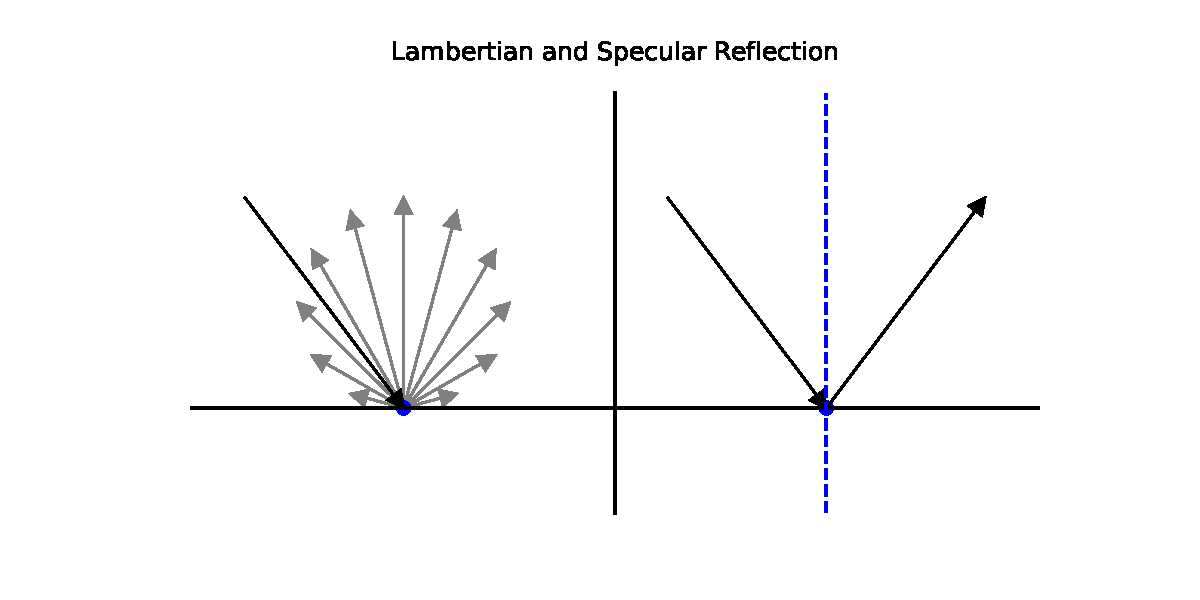
\includegraphics[scale = 0.4]{LambertSpec.pdf}
\centering
\caption{Lambertian and specular reflection diagram highlighting the difference between the two. Lambertian is left, specular is right. The ideal cases are pictured, real surfaces will deviate or even be a combination of the two. Our code assumes ideal behavior.}
\label{fig:1}
\end{figure}

Unfortunately, current radiative transfer models of Titan's atmosphere assume a rough, lambertian surface, perhaps with variable albedo \citep{Griffith2012, Xu2013, Corlies2021, Rannou2021, EsSayeh2023}. Yet, the difference between specular and lambertian surfaces in radiative transfer is significant. In order to properly model Titan, this difference needs to be accounted for; not only to ensure that our understanding of Titan's surface-atmosphere interaction is accurate, but also to assist in identifying unknown potentially-liquid terrain on Titan that has never had a favorable viewing geometry for direct specular reflections. 

In this paper, we demonstrate a specular reflection routine for SRTC++ (Spherical Radiative Transfer in C++), a radiative transfer code tailored to model Titan in the infrared wavelengths available to Cassini's VIMS (Visual and Infrared Mapping Spectrometer) instrument \citep{Barnes2018}. The new routine enables accurate simulation of liquid surfaces on Titan---in fact, as the properties of methane are well known, the accuracy for liquid surfaces is greater than that of the poorly-constrained land of Titan \citep{Trainer2018}. To demonstrate this routine, we begin with \textbf{Methods}, describing in brief the code and model we chose. \textbf{Results} examines the direct output of the completed simulation, and \textbf{Validation} compares those results to known lakes and seas on Titan. The implications of our simulation are considered in the \textbf{Discussion} before we end with a \textbf{Summary and Conclusion}.

\textbf{\color{red} [NOTE: Be sure to redo this last introduction paragraph when the paper is done.] \color{black}}

\section{Methods} \label{sec:methods}

The primary code for our simulation, SRTC++, is described in detail elsewhere \citep{Barnes2018}. However, in order to describe the new routine, a brief overview is required. SRTC++ simulates radiative transfer in a Monte Carlo fashion, making it nondeterministic. Individual ``photon packets'' are launched toward Titan, with the results of every scattering event in the atmosphere determined randomly. The detector objects in SRTC++ do not detect these ``photon packets'', but rather the result of their scattering events. Each scattering event has a certain probability of going any individual direction; SRTC++ finds the directions that go to the detectors and determines the intensity the detector would see from that event. Often, millions of ``photon packets'' are run for a single simulation, with each stattering event updating the detectors until a full picture of Titan forms at each detector.

In SRTC++, the ground is normally modeled as just another scattering event, just one with different probabilities than an atmospheric scatter \citep{Barnes2018}. This works well for rough, lambertian surfaces, where the distribution is quite random at macro scales. However, specular surfaces do not fit this mold, as light reflecting off of them follows a deterministic path.  The new routine takes advantage of this, calculating two different paths to the detector from every scattering event; one that goes directly to the scatter, and one that bounces off a specular surface first. This does leave a hole in the simulation: ``photon packets'' that pass through the atmosphere and strike the surface without scattering are missed. Fortunately, these missed packets would be at or near the point where the specular reflection is brightest and nowhere else, so minimal information about viewing geometry is lost. Furthermore, if recorded, those points would far outshine anything else in the resulting images, making them difficult to parse; just like real images of direct specular reflections on Titan, which are quite saturated \citep{Barnes2013}.

\begin{figure}[htbp]
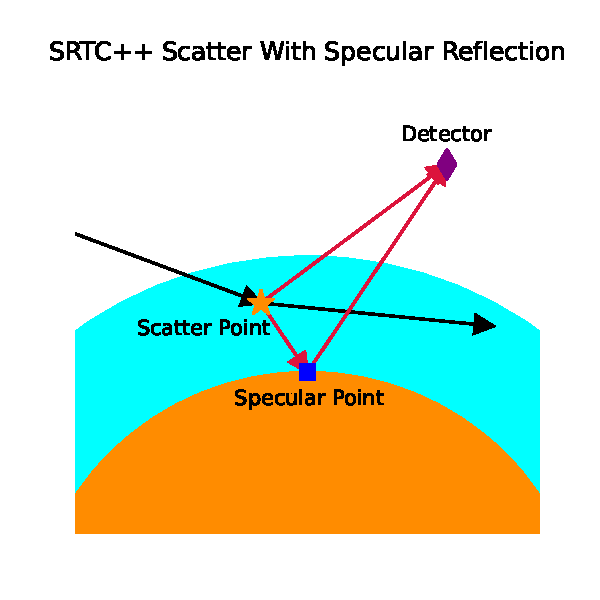
\includegraphics[scale = 0.55]{SRTCSpec.pdf}
\centering
\caption{SRTC++ operation with specular point. Photon packet comes in from the left on a black arrow, hitting the scatter point. The code determines both paths to the detector, shown with red arrows. One path is direct, the other reflects off the specular point on the surface. The photon packet itself will continue along the black arrow, potentially to scatter again.}
\label{fig:2}
\end{figure}

\begin{figure}[htbp]
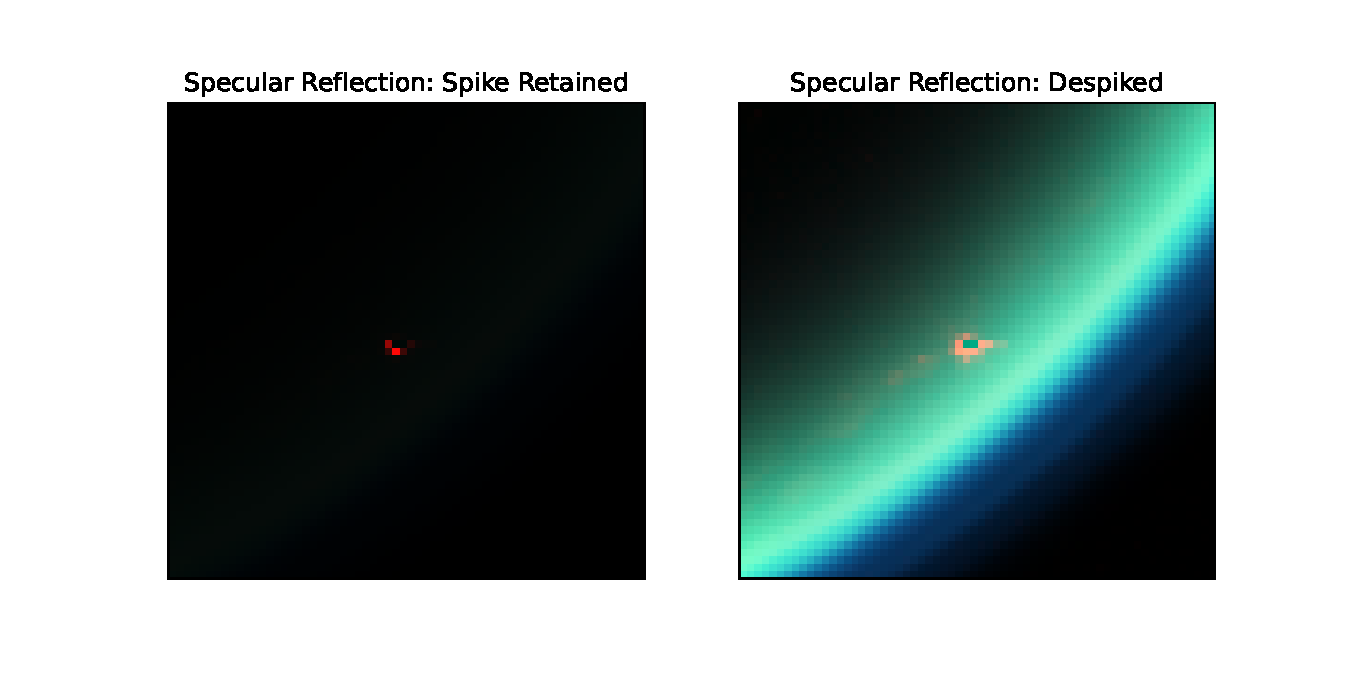
\includegraphics[scale = 0.35]{SpecSpikeNoSpike.pdf}
\centering
\caption{Cassini VIMS observation of specular reflection. CM\_1721848119\_1 on flyby T85. RGB map is to 5, 2, and 1.3 $\mu$m without any artificial scaling of individual colors. Left: resulting image retaining the spike values as 1, the maximum. Right: resulting image with trimmed spike values, set to 1. The specular reflection's spike is so dramatic it not only drowns out all other wavelengths, but it also outshines secondary reflections in the same wavelength, which contain valuable information. The hole in the center of the reflection is due to saturation of the VIMS instrument, indicating the real intensity of the direct specular reflection is beyond what we show here.}
\label{fig:3}
\end{figure}

The angle of the second ``photon packet'' path is determined both by the curved geometry of Titan's surface and the index of refraction of liquid methane. This new path can be ignored if the surface doesn't have liquid at the required location, however we will not make use of this ability in this paper as our chosen model is a global methane ocean. This model does not accurately represent Titan, but it does not have to: when we model a global methane ocean, we see the surface from almost every possible viewing geometry. This will enable us to compare the specular results to a lambertian simulation, quantifying the differences, which can in turn be used to characterize real surface observations. 

Titan is known to have at least some ethane in its seas \citep{Mastrogiuseppe2016} but the indeces of refraction of liquid methane and ethane are extremely similar \citep{Kanjanasakul2020}. We ran a simulation with ethane's index and noticed no clear differences between it and the methane result, qualitatively justifying the use of a pure methane ocean model. This also justifies not modeling the change of index of refraction with wavelength and our using a value that, strictly speaking, is slightly too low for the environmental conditions on Titan \citep{Martonchik1994, Jennings2019}. For a quantitative justification, we used the Fresnel equations to find the average reflection coefficient for water, ethane, and methane. Two methane values were examined, the one used in the code, and one sampled for more realistic Titan enviornmental conditions \citep{Martonchik1994}. The results of this are seen in Figure \ref{fig:4}. As the maximum variation between the two values of methane is ~2\%, we deem the variation neglegible. This also justifies not giving each tested wavelength of light a different index of refraction.

\begin{figure}[htbp]
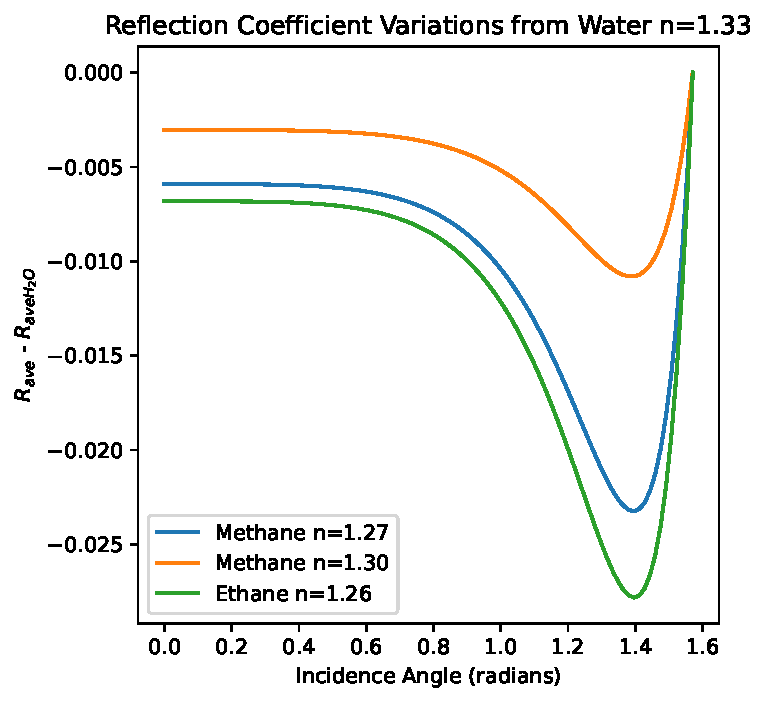
\includegraphics[scale = 0.5]{ReflectionVariations.pdf}
\centering
\caption{Average reflection coefficient differences from water with a 1.33 index of refraction. We do not plot the direct reflection coefficients since the differences between the various materials are largely indistinguishable. Methane 1.27 was used in the code, while methane 1.30 is more realistic. Note that the differences between the two are, across most angles, less than a percent, with a maximum difference of ~2\%. The mixture of ethane in Titan's lakes and seas will likely lower this difference even further. At large angles the difference approaches zero as all reflection coefficients approach unity.}
\label{fig:4}
\end{figure}

\textbf{\color{red} [NOTE: Perhaps all this justification would be better placed in an Appendix?] \color{black}}

No model of Titan is sufficient without an amosphere. SRTC++ primarily uses \cite{Tomasko2008} for Titan's atmosphere, and here we add corrections from \cite{Hirtzig2013} and \cite{Rodriguez2018}. The version of SRTC++ used does not account for atmospheric absorption, but such effects are expected to be limited at the wavelengths we are simulating \citep{EsSayeh2023}.

We compare our results to lambertian simulation data taken from (Barnes, in preparation), also created using SRTC++. We made sure that the input parameters matched between the two simulations. There are 72 detectors placed every 5$^{\circ}$ around Titan's equator at a distance of 10$^6$ km. Each detector sees 3500 km out from Titan's center, chosen to be significantly larger than Titan's 2575 km radius to avoid any edge artifacts.

\begin{figure}[htbp]
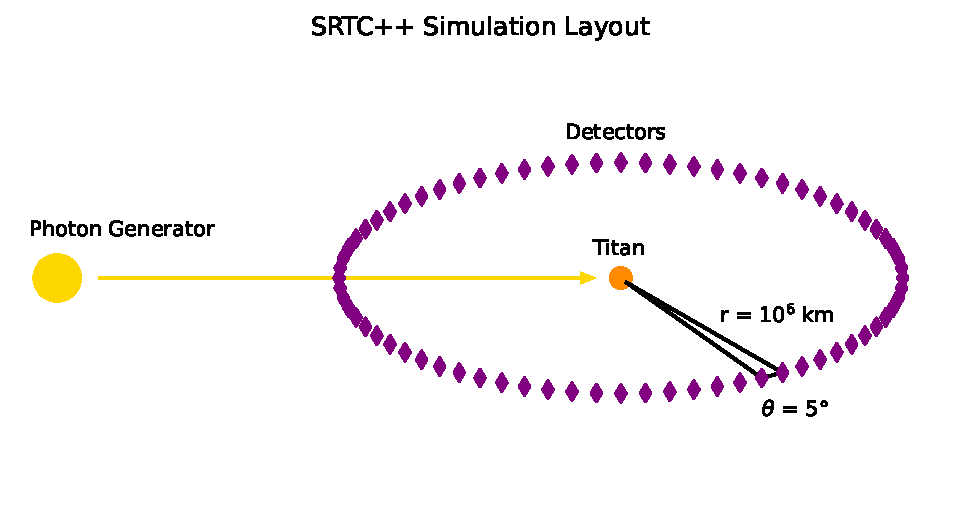
\includegraphics[scale = 0.5]{SRTCLayout.pdf}
\centering
\caption{Layout of our SRTC++ simulations, identical for both the specular and lambertian case. Distances not to scale. Detectors all equidistant from Titan and angular separation is the same for each one. The yellow arrow represents "photon packets" being shot at Titan. Note that it does not interact with the detector it passes through.}
\label{fig:5}
\end{figure}

Each simulation is run at eight different wavelengths that correspond to the eight atmospheric windows, areas of the electromagnetic spectrum that pierce through Titan's atmosphere and allow characterization of the surface \citep{Barnes2007}. Simulations could be run at other wavelengths, but they would mask any surface signals and be of minimal use for our current purposes. 

\section{Results} \label{sec:results}

\begin{figure}[htbp]
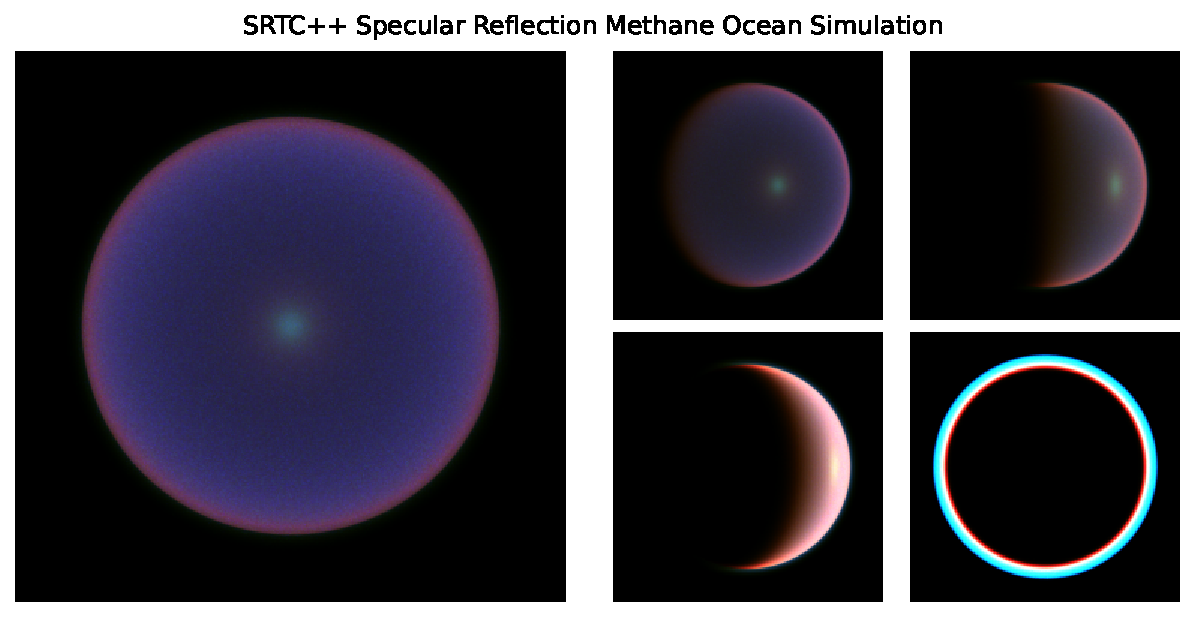
\includegraphics[scale = 0.4]{SpecularSim.pdf}
\centering
\caption{Simulation results for a methane ocean Titan, colored with 5, 2 and 1.3 $\mu$m mapped to red, green, and blue respectively. Left image is viewed at 0$^{\circ}$  from the incidence angle. Right four images are at  35$^{\circ}$ ,  90$^{\circ}$ ,  120$^{\circ}$ , and  180$^{\circ}$  in left to right then top to bottom order. \textbf{\color{red} [An animating version of the figure will exist in places that support it. The large left panel will hold the animating image, the right panels will remain static for comparisons] \color{black}}}
\label{fig:6}
\end{figure}

In \ref{fig:6} we have collected the results at 5, 2, and 1.3 $\mu$m mapped to red, green, and blue respectively in the same manner as \cite{Barnes2018}'s "surface spectral diversity" color scheme. The most obvious distinction between real images of Titan and this simulation is the color; most real Titan images done in this color scheme come out green or green-blue with some yellowish features. This is to be expected, as Titan is not a global methane ocean. The sharp blue component arises because pure methane's index of refraction does not vary significantly through the tested wavelengths \citep{Martonchik1994}, and so the atmosphere alone determines the color dependence. Since smaller wavelengths scatter more on Titan \citep{EsSayeh2023} the image appears bluer. The magenta coloration on the limb arises because the red channel, 5 $\mu$m, is enhanced in this color scheme and focuses most of its intensity on Titan's limb. We expect that it Titan really were a global methane ocean, it would look similar to the simulation, but we shall hold discussion of this until the Validation seciton.

The other primary features of the simulation are expected. The bright central area is near the specular point, caused by ``photon packets'' that nearly passed through the atmosphere unhindered, and so did not get scattered far from the ideal path. The circular shape of this feature flattens as it approaches the limb of Titan, which is what should occur on a slanted reflective surface. The limb brightening effect is due to refleciton coefficients rising as we approach 120$^{\circ}$ as seen in \ref{fig:4}. Toward the terminator, Titan appears redder because shorter wavelengths scatter away more readily, leaving only long wavelengths behind.

The simulation also produces ``eclipse views'' of Titan backlit by the sun, but those show the atmosphere and not the surface (for the most part), and so are beyond the scope of this paper. There is certainly worthwhile information to be gleaned here at a later date, though. 

\begin{figure}[htbp]
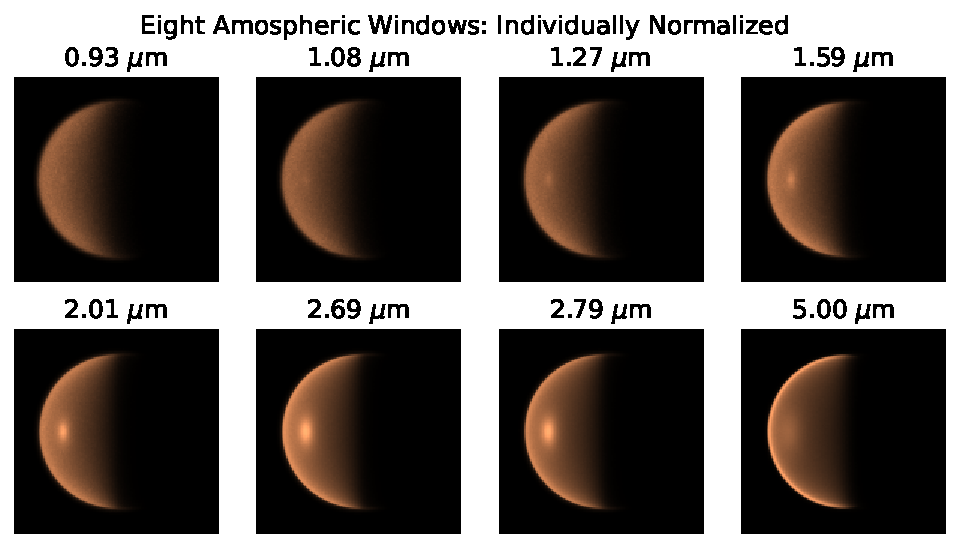
\includegraphics[scale = 0.5]{8WindowsNorm.pdf}
\centering
\caption{Individual wavelength simulated views of Titan for all eight atmospheric windows. Each image is individually normalized; in reality the short wavelengths are significantly brighter than the long ones. As wavelength increases, the sharpness of the near-specular area increases, up until the unusual case of 5 $\mu$m which is discussed in the text.}
\label{fig:7}
\end{figure}
\begin{figure}[htbp]
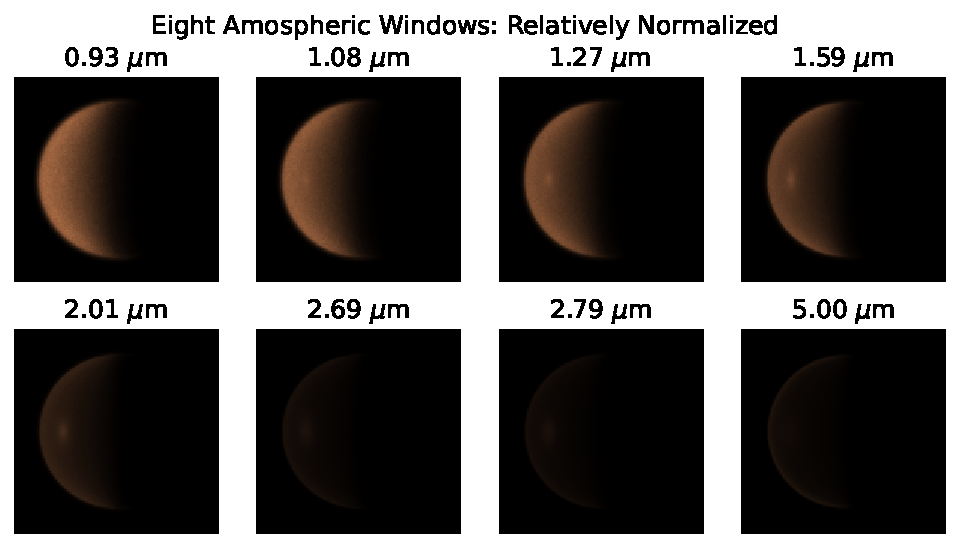
\includegraphics[scale = 0.5]{8WindowsNoNorm.pdf}
\centering
\caption{Same as \ref{fig:7} except that the images are scaled relative to each other. The longer wavelengths are so dim as to be essentially invisible. The 5 $\mu$m window is once again unusual, as it is actually brighter than the shorter wavelengths preceding it. See text for discussion.}
\label{fig:8}
\end{figure}

In truth, all eight of Titan's near-infrared atmospheric windows were simulated, not just the three used to create the color figures. \ref{fig:7} and \ref{fig:8} show a selection of images for all the simulated wavelengths.

In general, shorter wavelengths are more intense than longer ones. Shorter wavelengths are also noisier. Both of these facts have the same explanation: short wavelengths scatter more readily, making photons more likely to contribute to detectors while also scrambling information due to mutliple scattering events on a single "photon packet." This is also why the near-specular area is sharp in most longer wavelengths, but blurred out in shorter.

The brightness pattern is not followed perfectly: 5 $\mu$m is slightly brighter than 2.8 $\mu$m while also having a fuzzier near-specular area. This is an atmospheric effect, as all wavelengths are treated the same in this model. At 5 $\mu$m the atmosphere is known to have a very low optical depth; significantly lower than the other windows \citep{EsSayeh2023}, but this should make it dimmer rather than brighter. The true difference lies in the difference in the phase function between 5 $\mu$m and the other windows: both are forward scattering phase functions, but 5 $\mu$m is less so \citep{Tomasko2008}. This will force the light to take more distributed and indirect paths. Most visible paths in our images are from such viewing geometries, so with a significant difference in phase function, the overall appearance of Titan will increase in brightness. A side effect of this is that the viewing geometries that are close to direct forward scattering are going to be more diffuse than expected, which explains why the near-specular area at 5 $\mu$m isn't as bright or sharp as 2.8 $\mu$m. Similar reasons explain the enhanced limb brightness for 5 $\mu$m.

\begin{figure}[htbp]
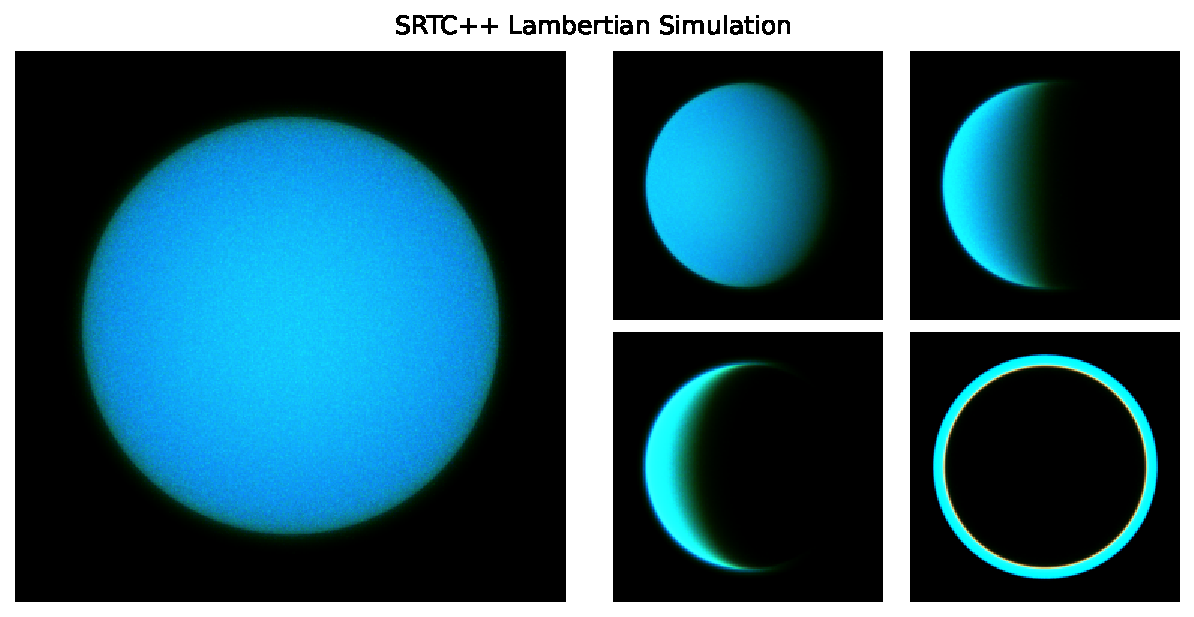
\includegraphics[scale = 0.4]{LambertianSim.pdf}
\centering
\caption{Simulation results for a lambertian Titan, colored with 5, 2 and 1.3 $\mu$m mapped to red, green, and blue respectively. Left image is viewed at 0$^{\circ}$  from the incidence angle. Right four images are at  35$^{\circ}$ ,  90$^{\circ}$ ,  120$^{\circ}$ , and  180$^{\circ}$  in left to right then top to bottom order. \textbf{\color{red}[An animating version of the figure will exist in places that support it. The large left panel will hold the animating image, the right panels will remain static for comparisons] \color{black}}}
\label{fig:9}
\end{figure}

Direct comparisons between the specular and lambertian simulations (Barnes, in preparation) reveal a few key differences. First, the lambertian simulation is brighter than the specular everywhere except near the specular point \textbf{\color{red} [Check with actual intesnity values to be sure] \color{black}}. This was expected, each simulation's Titan is receiving the same amount of energy, but the specular Titan will preferentially focus its light in a single direction, while the lambertian will not, leading the specular point and areas near it to be bright in the specular simulation while everywhere else is relatively dim. 

The overall coloration of both simulations is similar, with blue and magenta taking prominent roles. However, the distribution of these colors is markedly different, with the lambertian simluation's disc being mostly magenta rather than blue. When light encounters a lambertian surface it scatters in a random direction, which means any time a "photon packet" hits the ground, it could easily be sent right to a detector. This is not so in the specular simulation, so the specular detector has to rely on atmospheric scattering to send light its way and the atmosphere scatters bluer light more readily. Ultimately, this is also the reason the lambertian simulation doesn't have a noticable near-specular glare.

The lambertian simulation has a lesser limb brightening effect at low phase as it has no index of refraction. Strong limb brightening can still be seen at higher phase, but this is due to the atmosphere, as the specular simulation also showcases this increasing limb brightening with higher phase.

The eclipse views in both simulations are virtually identical. As they should be, since the atmosphere model for both is the same.

Details on the interpretation of the lambertain simulation on its own can be found in (Barnes, in preparation). 

So far, we have only considered qualitative differences between the specular and lambertian geometries. For quantitative analysis, we chose to deconstruct the simulation data by viewing geometry. We took every single simulation pixel that showed the surface (as opposed to the atmosphere) and determined the incidence, emission, and azimuth angles. Any viewing gometries that were hit more than once were added together and then averaged. The result was a database in incidence, emission, azimuth, and wavelength that showed the intensity \textbf{\color{red}[I have GOT to nail down what the exact words and units are that we're simulating]\color{black}} at every possible geometry. We then subtracted the lambertian value from the specular one.

\begin{figure*}[htbp]
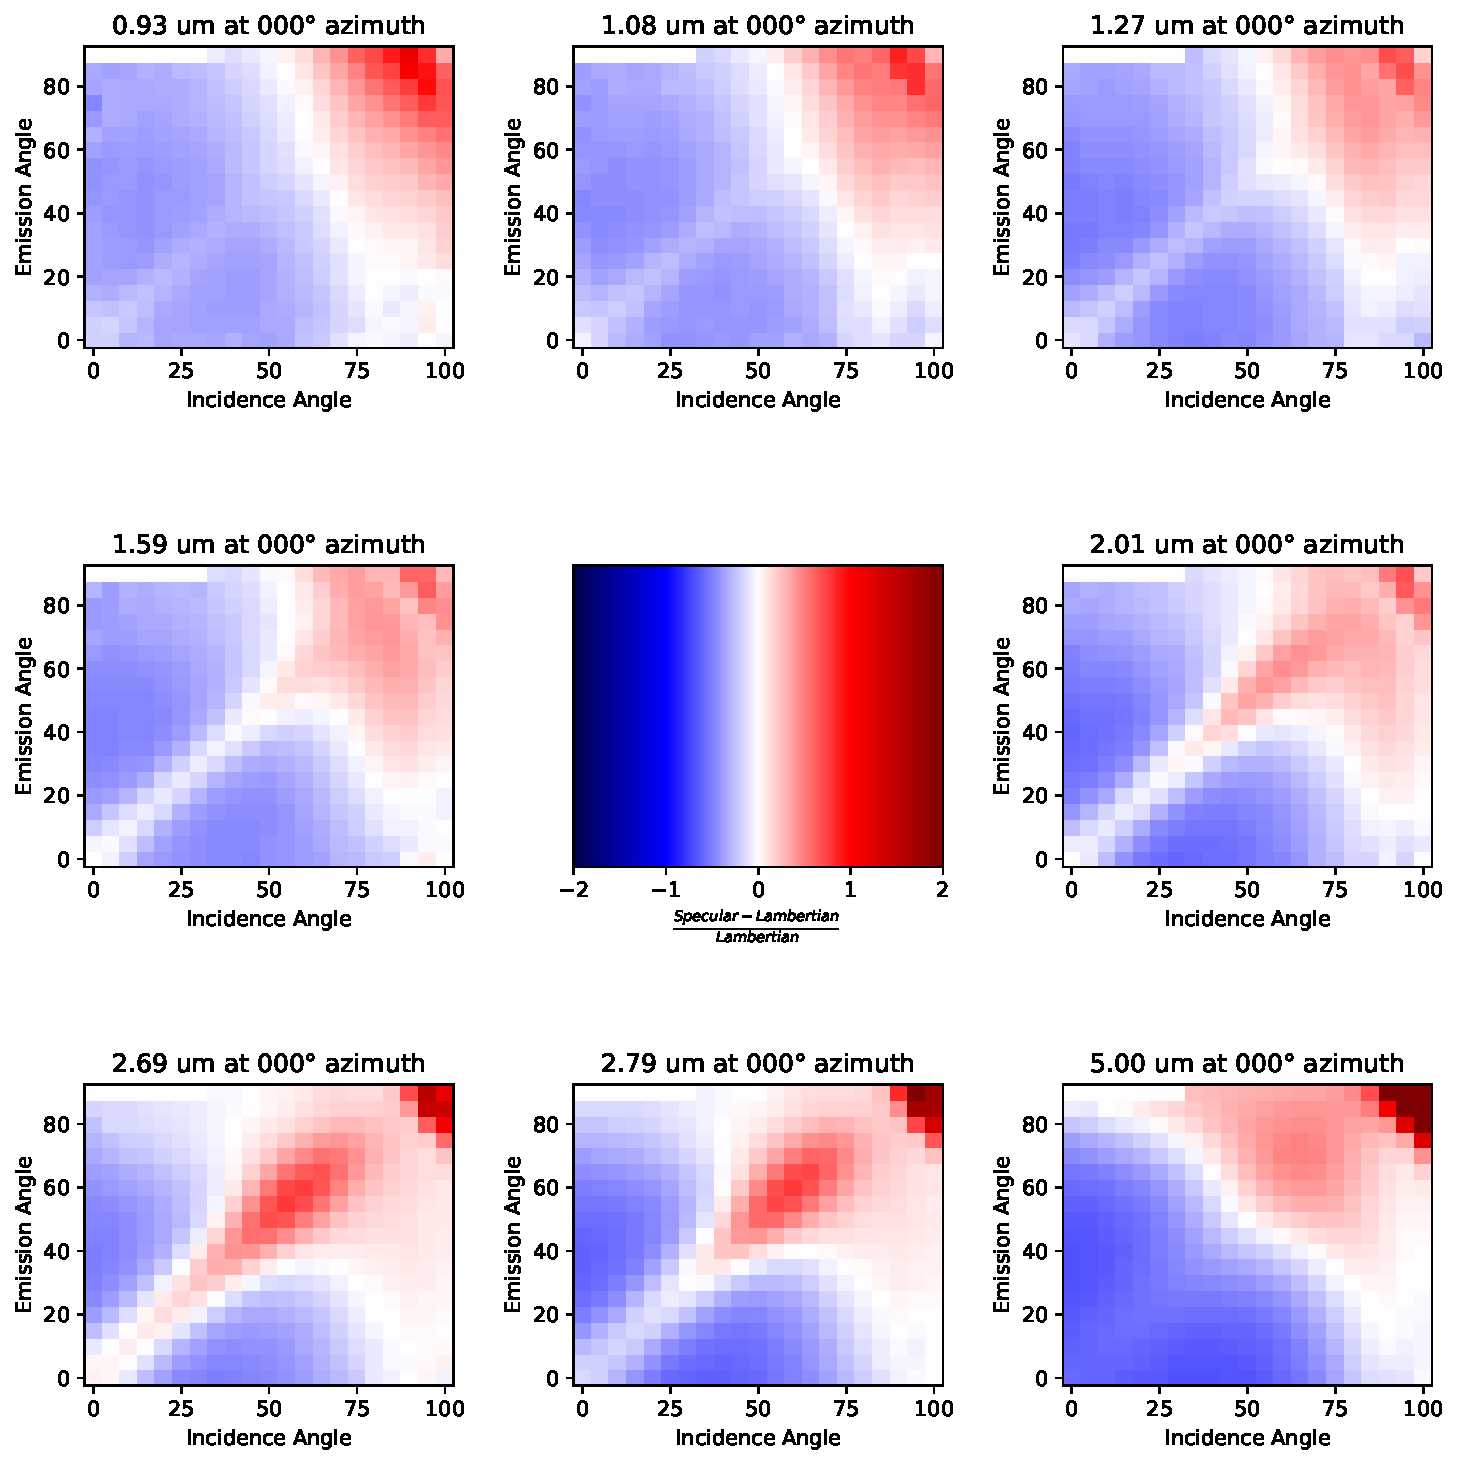
\includegraphics[scale = 0.54]{SpecLambNormDiff.pdf}
\centering
\caption{Comparison of specular and lambertian simulations based on viewing geometry. Each of the eight exterior plots are at one wavelength, with the horizontal and vertical axes plotting incidence and emission angle respectively. Negative (blue) values are where the lambertian simulation is brighter, while positive (red) values are where specular dominates. The behavior can be broadly categorized into three types: short wavelength, long wavelength, and 5 $\mu$m. \textbf{\color{red} [An animating version of the figure will exist in places that support it. The eight wavelength panels will cycle through all of the azimuth angles in time.] \color{black}}}
\label{fig:10}
\end{figure*}

The broad behavior of \ref{fig:10} is expected: we see that lambertian dominates in the negative (blue) areas, which take up most of the viewing geometries, matching what we saw visually. Specular dominantes in the positive (red) areas, which cluster around places where emission and incidence match (near the specular point) and places with high emission and incidence (limb effects). These two are easily explained with specular reflection and total reflection from the index of refraction, respectively.

A cursory inspection of \ref{fig:10} reveals three distinct types of behavior: the three shortest wavelengths, the four longer wavelengths, and 5 $\mu$m in its own class. The three shortest wavelengths tend not to dominate near the specular point due to noise clearly visible in \ref{fig:7}. Do note that in a real image of Titan, the direct specular reflection would change this, but only for viewing geometries very close to the specular point. The longer wavelength class simply has a clear near-specular area that isn't blocked by noise. Both classes dominate at the limb. 

Notably, the behavior of the 5 $\mu$m is distinctly different than the other windows, with a distinctly different shape and gradient across the azimuth. This is, in general, expected, as 5 $\mu$m is a much wider window separated from the other windows by a significant portion of the electromangetic spectrum \citep{EsSayeh2023}. In fact this difference may be supremely helpful, as the behavior of the 5 $\mu$m window with respect to the others at different viewing angles could potentially be used as a test to identify liquid bodies. 

Of course, actually making use of the differences in specular and lambertian behavior depends on validation. We expect the specular model to be accurate for large bodies of liquid methane, and we have plenty of viewing geometries from the Cassini mission to test.

\section{Validation} \label{sec:validation}

As has been mentioned multiple times in this paper, we expect the methane ocean simulated to be a reasonable approximation of reality. We are in such a situation that we can demonstrate this by comparing the simulation to real Cassini VIMS data of the seas of Titan. (For validation of the lambertian simulation, see (Barnes, in preparation) \textbf{\color{red} Though is it right to call it validation if we don't expect it to match reality? \color{black}}). 

We restrict our initial validation to the inner portions of Titan's seas, to avoid any contamination from the solid shore and give us the largest data set. We also consider Ontario Laucus despite its small size and limited data set, as it is the only body of water on the southern pole. 

\color{blue}Known lakes... perhaps also land next to the lakes... table of used flybys/locations... visual comparison first, then qualitative... really hope the validation confirms what we have... demonstrate ``identification'' of a lake using the data in the previous section... \color{black}

\textbf{\color{red}[Validation procedure: compare with known lakes. Explain selection process for which images/flybys we used for this (not that I know what this procedure is yet, as we haven't even started this part). Show a visual comparison first, then a quantitative comparison. (Structure: once per flyby used? Once per feature? Or do all visual comparisons and then all quantitative ones?) Compare the quantitative differences and assign some kind of confidence value as to how close our model is to reality. We HOPE that this validation is confirmed. If it is not we presumably need to go back to the drawing board and figure out what went wrong rather than publishing this paper. (if it goes wrong it's possibly a lack of absorption or some other feature.)]]\color{black}}

\section{Discussion} \label{sec:discussion}

Lorem ipsum dolor sit amet, consectetur adipiscing elit, sed do eiusmod tempor incididunt ut labore et dolore magna aliqua. Ut enim ad minim veniam, quis nostrud exercitation ullamco laboris nisi ut aliquip ex ea commodo consequat. Duis aute irure dolor in reprehenderit in voluptate velit esse cillum dolore eu fugiat nulla pariatur. Excepteur sint occaecat cupidatat non proident, sunt in culpa qui officia deserunt mollit anim id est laborum.

\textbf{\color{red}[So we don't know what to put here really since we haven't done the full experiment. Most of the observations I currently know of are best put in Results as they are observations about the results directly rather than any real new knowledge. If validation flies, we do have one piece of knowledge: to find lakes look for fully illuminated disks and find the BLUE in Jason Color. Other possible dicsussion points: deviations from reality, noise at five microns, error quantifications if we can get them, other potential signs of lakes. FUTURE WORK: methods for identifying specular stuff.]
\color{black}}

Perhaps the most obvious way to differentiate specular from lambertian surfaces on Titan is to look at pictures where both types are present at different viewing angles, and see how they change. This is helpful for validating the model against known lakes, but is unhelpful for identifying new ones. The primary issue is that while the methane ocean is expected to be an accurate representation of reality, the idealized lambertian surface is not. After all, real VIMS images of titan are greenish, not pinkish. 

\color{blue} LEFTOVERS FROM RESULTS: In order to identify bodies... challenges from inaccuracy of lambertian versus accuracy of specular... need multiple reference points at different viewing angles... find the most dramatic viewing angle changes... maybe go based on viewing angles of location... genrealize? Lots of unknowns. \color{black}

\section{Summary and Conclusion} \label{sec:conclusion}

Lorem ipsum dolor sit amet, consectetur adipiscing elit, sed do eiusmod tempor incididunt ut labore et dolore magna aliqua. Ut enim ad minim veniam, quis nostrud exercitation ullamco laboris nisi ut aliquip ex ea commodo consequat. Duis aute irure dolor in reprehenderit in voluptate velit esse cillum dolore eu fugiat nulla pariatur. Excepteur sint occaecat cupidatat non proident, sunt in culpa qui officia deserunt mollit anim id est laborum. 

\textbf{\color{red}[Conclude based on how confident we are in the simluation, and summarize points of new science and potential indications of how to identify future lakes. Keep it simple and short, but make sure to include relevant details, such as precise values that can be used to detect lakes. Summary of most important points is simply helpful to readers]]\color{black}}

\begin{acknowledgments}
Insert ACK here. 

\color{blue}Data availability? Would like to make it clear that we'll give all the information after just being asked...\color{black}

\textbf{\color{red}[Not sure who needs to be put here who won't be put on the author list. Though there is going to be funding recongition here.]\color{black}}
\end{acknowledgments}

\appendix

\section{Appendix?}

Appendix!

\bibliography{Bibliography}{}
\bibliographystyle{aasjournal}

\end{document}